% \vspace{-0.8cm}
\section{Experiment}\label{sec:experiment}
In experiments, we aim to address the following research questions: (1) How does \ourmethod perform in multi-hop retrieval and QA tasks? (\Cref{sec:retrieval,sec:qa}); (2) What are the efficiency and effectiveness of \ourmethod in multi-hop retrieval? (\Cref{sec:efficiency}); (3) How well does \ourmethod generalize to unseen datasets as a foundation model? (\Cref{sec:generalizability}); (4) How does the performance of \ourmethod scale with training as a foundation model? (\Cref{sec:scaling}); (5) How to interpret \ourmethod in multi-hop reasoning? (\Cref{sec:interpretation}).

% \vspace{-0.4cm}
\subsection{Experimental Setup}\label{sec:setup}
\noindent\textbf{Datasets.} We first evaluate the effectiveness of \ourmethod on three widely-used multi-hop QA datasets, including HotpotQA \citep{yang2018hotpotqa}, MuSiQue \citep{trivedi2022musique}, and 2WikiMultiHopQA (2Wiki) \citep{ho2020constructing}. We also evaluate the performance of \ourmethod on seven RAG datasets from three domains, including biomedical \citep{jin-etal-2019-pubmedqa}, custom support \citep{sadat-etal-2023-delucionqa,nandy-etal-2021-question-answering,malaviya2023expertqa,castelli-etal-2020-techqa}, and general knowledge \citep{nguyen2016ms,kamalloo2023hagrid}, to demonstrate the generalizability of \ourmethod as the foundation model. The detailed statistics of the test datasets are shown in the \Cref{app:datasets}.

\noindent\textbf{Baselines.} We compare against several widely used retrieval methods under three categories: (1) \emph{single-step naive methods}: BM25 \citep{robertson1994some}, Contriever \citep{izacardunsupervised}, GTR \citep{ni2022large}, ColBERTv2 \citep{santhanam2022colbertv2}, RAPTOR \citep{sarthiraptor}, Proposition \citep{chen-etal-2024-dense}; (2) \emph{graph-enhanced methods}: GraphRAG (MS) \citep{edge2024local}, LightRAG \citep{guo2024lightrag}, HippoRAG \citep{gutiérrez2024hipporag}, SubgraphRAG~\citep{lisimple}, G-retriever~\citep{he2024g}; (3) \emph{multi-step methods}: Adaptive-RAG \citep{jeong2024adaptive}, FLARE \citep{jiang2023active}, and IRCoT \citep{trivedi2023interleaving} framework that can be integrated with arbitrary retrieval methods to conduct multi-step retrieval and reasoning. The detailed introduction of the baselines are shown in the \Cref{app:baselines}.

\noindent\textbf{Metrics.} For retrieval performance, we use recall@2 (R@2) and recall@5 (R@5) as evaluation metrics. For final QA performance, we use the EM score and F1 score following previous works \citep{gutiérrez2024hipporag}.

\noindent\textbf{Implementation Details.} 
The GFM retriever is implemented with 6 query-dependent message passing layers with the hidden dimension set to 512. The pre-trained all-mpnet-v2 \citep{all-mpnet-v2} is adopted as the sentence embedding model and is frozen during training. The total parameters of the GFM retriever are 8M, which is trained on 8 NVIDIA A100s (80G) with batch size 4, learning rate 5e-4, and loss weight $\alpha=0.3$. The training data contains 60 KGs with over 14M triples constructed from 700k documents extracted from the training set. 
The statistics of training data are shown in \Cref{tab:training_data}, and the implementations are detailed in \Cref{app:implementation}.

% \subsection{Experimental Setup}\label{sec:setup}
% \noindent\textbf{Datasets.} We first evaluate the effectiveness of \ourmethod on three widely-used multi-hop QA datasets, including HotpotQA \citep{yang2018hotpotqa}, MuSiQue \citep{trivedi2022musique}, and 2WikiMultiHopQA (2Wiki) \citep{ho2020constructing}. For a fair comparison \citep{trivedi2023interleaving,gutiérrez2024hipporag}, we use 1,000 samples from each validation set for testing. We merge the candidate passages into the document corpus and extract 20,000 samples from each training set for GFM training. We also evaluate the performance of \ourmethod on seven RAG datasets from three domains, including biomedical \citep{jin-etal-2019-pubmedqa}, custom support \citep{sadat-etal-2023-delucionqa,nandy-etal-2021-question-answering,malaviya2023expertqa,castelli-etal-2020-techqa}, and general knowledge \citep{nguyen2016ms,kamalloo2023hagrid}, to demonstrate the generalizability of \ourmethod as the foundation model. The detailed statistics of the test datasets are shown in the \Cref{app:datasets}.

% \noindent\textbf{Baselines.} We compare against several widely used retrieval methods under three categories: (1) \emph{single-step naive methods}: BM25 \citep{robertson1994some}, Contriever \citep{izacardunsupervised}, GTR \citep{ni2022large}, ColBERTv2 \citep{santhanam2022colbertv2}, RAPTOR \citep{sarthiraptor}, Proposition \citep{chen-etal-2024-dense}; (2) \emph{graph-enhanced methods}: GraphRAG (MS) \citep{edge2024local}, LightRAG \citep{guo2024lightrag}, HippoRAG \citep{gutiérrez2024hipporag}; (3) \emph{multi-step methods}: Adaptive-RAG \citep{jeong2024adaptive}, FLARE \citep{jiang2023active}, and IRCoT \citep{trivedi2023interleaving} framework that can be integrated with arbitrary retrieval methods to conduct multi-step retrieval and reasoning. The detailed introduction of the baselines are shown in the \Cref{app:baselines}.

% \noindent\textbf{Metrics.} For retrieval performance, we use recall@2 (R@2) and recall@5 (R@5) as evaluation metrics. For the final QA performance, we use the EM score and F1 score following previous works \citep{gutiérrez2024hipporag}.

% \noindent\textbf{Implementation Details.} The GFM retriever\footnote{\url{https://anonymous.4open.science/r/deep_graphrag-24D6}} is implemented with 6 query-dependent message passing layers with the hidden dimension set to 512. The pre-trained all-mpnet-v2 \citep{all-mpnet-v2} is adopted as the sentence embedding model and is frozen during training. The total parameters of the GFM retriever are 8M, which is trained on 8 NVIDIA A100s (80G) with batch size 4, learning rate 5e-4, and loss weight $\alpha=0.3$. The training data contains 60 KGs with over 14M triples constructed from 700k documents extracted from the training set. The statistics are shown in \Cref{tab:training_data}, and the detailed data construction process, model settings, and training process are shown in \Cref{app:implementation}.

% \vspace{-0.3cm}

\input{tables/retrieval_performance.tex}
\subsection{Retrieval Performance}\label{sec:retrieval}
We first evaluate the retrieval performance of \ourmethod against the baselines on three multi-hop QA datasets. As shown in \Cref{tab:retrieval}, \ourmethod achieves the best performance on all datasets, outperforming the SOTA IRCoT + HippoRAG by 16.8\%, 8.3\%, 19.8\% in R@2 on HotpotQA, MuSiQue, and 2Wiki, respectively. The results demonstrate the effectiveness of \ourmethod in multi-hop retrieval. From the result, we can observe that the naive single-step retrievers (e.g., BM25, RAPTOR) are outperformed by graph-enhanced HippoRAG, which highlights the significance of graph structure in multi-hop retrieval. Although GraphRAG (MS) and LightRAG use the graph structure, it struggles with multi-hop QA tasks as its retriever is designed for summarization and lacks multi-hop reasoning capability.
With the help of LLMs, the multi-step retrieval pipeline IRCoT improves the performance of all single-step methods through iterative reasoning and retrieval. However, \ourmethod still outperforms the multi-step methods by a large margin even with a single-step retrieval. This indicates that the \ourmethod can effectively conduct the multi-hop reasoning in a single step (detailed in \Cref{sec:interpretation} and \Cref{app:multi_hop}), which is more efficient and effective than the multi-step retrieval pipeline (detailed in \Cref{sec:efficiency}).

\subsection{Question Answering Performance}\label{sec:qa}
% \begin{wraptable}{r}{0.6\columnwidth}
\begin{table}
    \centering
   %  \vspace{-0.6cm}
    \caption{Question answering performance comparison.}
    \label{tab:qa}
    \resizebox{.9\columnwidth}{!}{%
    \begin{tabular}{@{}c|l|cc|cc|cc@{}}
    \toprule
    \multirow{2}{*}{Category}    & \multicolumn{1}{c|}{\multirow{2}{*}{Retriever}} & \multicolumn{2}{c|}{HotpotQA} & \multicolumn{2}{c|}{MuSiQue} & \multicolumn{2}{c}{2Wiki} \\ \cmidrule(l){3-8} 
                                 & \multicolumn{1}{c|}{}                           & EM            & F1            & EM            & F1           & EM          & F1          \\ \midrule
    \multirow{5}{*}{Single-step} & None                                            & 30.4          & 42.8          & 12.5          & 24.1         & 31.0        & 39.0        \\
                                 & ColBERTv2                                       & 43.4          & 57.7          & 15.5          & 26.4         & 33.4        & 43.3        \\
                                    & GraphRAG (MS) & 35.3 & 54.6 & 13.4 & 29.5 & 28.3 & 46.9 \\
                                 & LightRAG & 36.8 & 48.3 & 18.1 & 27.5 & 45.1 & 49.5 \\
                                 & HippoRAG (ColBERTv2)                            & 41.8          & 55.0          & 19.2          & 29.8         & 46.6        & 59.5        \\ \midrule
    \multirow{4}{*}{Multi-step}                                   & Adaptive-RAG & 45.5	& 59.6	& 13.8	& 25.6	& 48.9	& 62.8 \\
                                 & FLARE & 48.7 & 60.6 & 16.2 & 28.4 & 46.7 & 65.4 \\ 
    & IRCoT (ColBERTv2)                               & 45.5          & 58.4          & 19.1          & 30.5         & 35.4        & 45.1        \\
                                 & IRCoT + HippoRAG (ColBERTv2)                    & 45.7          & 59.2          & 21.9          & 33.3         & 47.7        & 62.7        \\ 
                                 \midrule
                                 Single-step                  & \ourmethod                                      & {\ul 51.6}    & {\ul 66.9}    & {\ul 30.2}    & {\ul 40.4}    & {\ul 69.8}    & {\ul 77.7}    \\
    Multi-step                   & IRCoT + \ourmethod                              & \textbf{56.0} & \textbf{71.8} & \textbf{36.6} & \textbf{49.2} & \textbf{72.5} & \textbf{80.8}       \\ \bottomrule
    \end{tabular}%
    }
   %  \end{wraptable}
   \end{table}
We then evaluate the QA performance of \ourmethod, as it is directly influenced by retrieval quality. We adopt the GPT-4o-mini \citep{gpt4o} as LLM and use the top-$5$ retrieved documents for generating answers. From the results shown in \Cref{tab:qa}, the single-step \ourmethod has already achieved state-of-the-art performance against all other baselines. Meanwhile, we also integrate \ourmethod with IRCoT to conduct multi-step retrieval and reasoning, which further improves the performance by 8.5\%, 21.2\%, 3.9\% in EM on three datasets, respectively. The results demonstrate the effectiveness and great compatibility of \ourmethod with an arbitrary multi-step framework in multi-hop reasoning tasks.

% \vspace{-0.3cm}
\subsection{Efficiency Analysis}\label{sec:efficiency}
% \begin{wraptable}{r}{0.6\columnwidth}
\begin{table}
    \centering
    % \vspace{-0.6cm}
    \caption{Retrieval efficiency and performance comparison.}
    \label{tab:efficiency}
    \resizebox{.8\columnwidth}{!}{%
        \begin{tabular}{@{}l|cc|cc|cc@{}}
            \toprule
            \multirow{2}{*}{Method} & \multicolumn{2}{c|}{HotpotQA} & \multicolumn{2}{c|}{MuSiQue} & \multicolumn{2}{c}{2Wiki}                                                  \\
                                    & Time (s)                      & R@5                          & Time (s)                  & R@5           & Time (s)       & R@5           \\ \midrule
            ColBERTv2               & \textbf{0.035}                & 79.3                         & \textbf{0.030}            & 49.2          & \textbf{0.029} & 68.2          \\
            HippoRAG                & 0.255                         & 77.7                         & 0.251                     & 51.9          & 0.158          & 89.1          \\
            LightRAG                & 0.861                         & 54.7                         & 1.109                     & 34.7          & 0.911          & 59.1          \\
            GraphRAG (MS)          & 2.759                         & 76.6                         & 3.037                     & 49.3          & 1.204          & 77.3          \\ \midrule
            IRCoT + ColBERTv2       & 1.146                         & 82.0                         & 1.152                     & 53.7          & 2.095          & 74.4          \\
            IRCoT + HippoRAG        & 3.162                         & 83.0                         & 3.104                     & 57.6          & 3.441          & 93.9          \\ \midrule
            \ourmethod              & {\ul 0.107}                   & \textbf{87.1}                & {\ul 0.124}               & \textbf{58.2} & {\ul 0.060 }   & \textbf{95.6} \\ \bottomrule
        \end{tabular}%
    }
    % \vspace{-0.5cm}
% \end{wraptable}
\end{table}
\ourmethod achieves great efficiency in performing multi-step reasoning in a single step. As shown in \Cref{tab:efficiency}, while the naive single-step methods get the best efficiency whose performance is not satisfying. Admittedly, the multi-step framework IRCoT could improve the performance, but it suffers from high computational costs due to the iterative retrieval and reasoning with LLMs. In contrast, \ourmethod conducts multi-hop reasoning within a single-step GNN reasoning, which is more effective than single-step methods and more efficient than multi-step ones.

% \vspace{-0.3cm}
\subsection{Ablation Study}\label{sec:ablation}
We conduct ablation studies to investigate the effectiveness of different components in \ourmethod, including: different sentence embedding models (\Cref{app:text_embeddings}), pre-training strategies (\Cref{app:pre-training}), loss weighting strategies (\Cref{app:loss_weight}), ranking methods (\Cref{app:ranking_method}), training datasets (\Cref{app:training_data_ablation}), and the construction of KG-index (\Cref{app:cost}). The results show that \ourmethod is not sensitive to different sentence embedding models, and the pre-training strategy, as well as the loss weighting strategy, are both crucial for the performance of \ourmethod.

% \vspace{-0.3cm}
% \input{figures/radar.tex}
\subsection{Model Generalizability}\label{sec:generalizability}
To demonstrate the generalizability of \ourmethod as a foundation model, we test the performance (R@5) of \ourmethod on seven RAG datasets without any domain-specific fine-tuning. Specifically, we first build the KG-index from the documents in each dataset. Then, given the query, we use the pre-trained GFM retriever to retrieve the top-$K$ documents with the help of the corresponding KG-index.
%
As shown in \Cref{fig:radar}, \ourmethod achieves the best performance on all datasets, outperforming the SOTA HippoRAG by 18.9\% on average. The results demonstrate the generalizability of \ourmethod as the foundation model which can be directly applied to various unseen datasets without any domain-specific fine-tuning. Additionally, results in \Cref{app:trans} demonstrate \ourmethod's strong transferability for further performance improvement when fine-tuned on domain-specific datasets.

\begin{figure}[t]
    \centering
    \begin{minipage}[t]{0.48\linewidth}
        \centering
        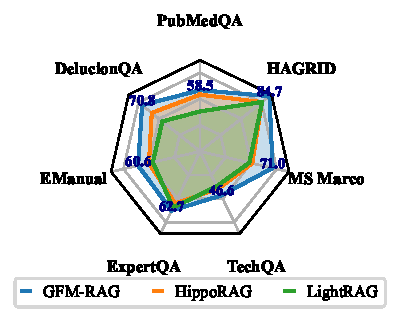
\includegraphics[width=1\linewidth]{images/radar.pdf}
        % \vspace{-0.4cm}
        \caption{Model generalizability comparison.}
        \label{fig:radar}
    \end{minipage}%
    \hfill
    \begin{minipage}[t]{0.48\linewidth}
        \centering
        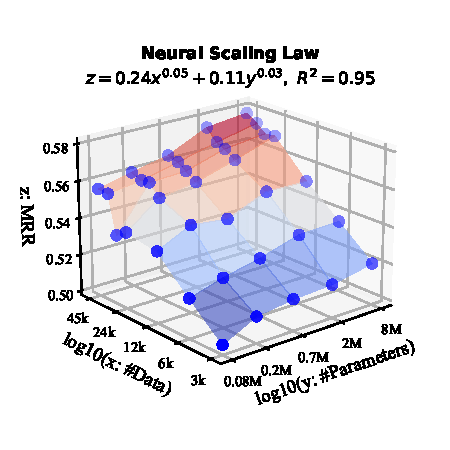
\includegraphics[width=1\linewidth]{images/scaling_law.pdf}
        % \vspace{-0.3cm}
        \caption{Neural scaling law of \ourmethod.}
        \label{fig:scaling}
    \end{minipage}
    % \vspace{-0.6cm}
\end{figure}


% \input{figures/scaling.tex}
\input{tables/path_cases.tex}
% \vspace{-0.3cm}
\subsection{Model Neural Scaling Law}\label{sec:scaling}
We further investigate the neural scaling law of \ourmethod, which quantifies how model performance grows with the scale of training data and model parameter size. It has been validated in the recent foundation models \citep{kaplan2020scaling,dehghani2023scaling}. As shown in \Cref{fig:scaling}, the performance of \ourmethod (MRR: $z$) scales well with the training data ($x$) and the model size ($y$), which can be fitted by the power-law scaling law $z \propto 0.24x^{0.05} + 0.11y^{0.03}$. The results demonstrate the scalability of \ourmethod as the foundation model and potential for further improvement. The detailed analysis of the neural scaling law is shown in \Cref{app:scaling}.

% \vspace{-0.2cm}
\subsection{Path Interpretations}\label{sec:interpretation}
\ourmethod exhibits the multi-hop reasoning ability powered by the multi-layer GFM. We provide path interpretations of \ourmethod for multi-hop reasoning in \Cref{tab:cases}. Inspired by NBFNet \citep{zhu2021neural}, the paths' importance to the final prediction can be quantified by the partial derivative of the prediction score with respect to the triples at each layer (hop), defined as:
\begin{equation}
    \setlength\abovedisplayskip{0pt}%shrink space
    \setlength\belowdisplayskip{0pt}
    s_1,s_2,\ldots,s_L=\arg\mathop{\text{top-}}k\frac{\partial p_e(q)}{\partial s_l}.
\end{equation}
The top-$k$ path interpretations can be obtained by the top-$k$ longest paths with beam search. We illustrate the path interpretations in \Cref{tab:cases}. In the first example, \ourmethod successfully deduces that the singer of the song has a football club named after him and that he owned it. In the second example, \ourmethod identifies two paths related to the murder case and the judge presiding over the trial. These interpretations show that \ourmethod exhibits the ability of multi-hop reasoning within single-step retrieval. We also illustrate the distribution the multi-hop prediction in \Cref{app:multi_hop}.